\documentclass[serif,xcolor=pdftex,dvipsnames,table,hyperref={bookmarks=false,breaklinks}]{beamer}

%%%%%%%%%%%%%%%%
% Change the macros below to configure the title slides
% for your course.
\newcommand{\coursename}{COMPSCI 590N}
\newcommand{\instructor}{Roy J. Adams}
\newcommand{\university}{University of Massachusetts Amherst}
\newcommand{\department}{College of Information and Computer Sciences}
%%%%%%%%%%%%%%%%

\newcommand\HUGE{\@setfontsize\Huge{50}{60}}

\newcommand{\settitlecard}[2]{
  \title[\coursename  Lecture #1] 
    {\coursename \\ Lecture #1: #2}
     \author[\instructor]{\instructor}
     \institute[\university]{
     \department\\
     \university
   }
\date{}
}

\newcommand{\maketitlepage}{
  \begin{frame}
  \titlepage
  %\center{
    %If you use the slides unmodified, retain the attribution below
  %  \tiny{Slides by Roy J. Adams (rjadams@cs.umass.edu). 
    %If you modify the slides, please retain the alternate attribution below
    %\tiny{Based on slides by Roy J. Adams (rjadams@cs.umass.edu). \\    
  %  }                                              
  %}  
  \end{frame}
}

\AtBeginSection[]
{
  \begin{frame}<beamer>{Outline}
    \tableofcontents[currentsection,subsectionstyle=hide]
  \end{frame}
}


\newcommand{\cut}[1]{}

\newcommand{\iconbox}[4]{
  \only<#1-#2>{
    \begin{columns}[T]
      \column{0.5in}
           \includegraphics[width=0.5in]{#3}
       \column{3.7in}
            #4
    \end{columns}
    \medskip
    \medskip
    \medskip
  }
}

\mode<presentation>{
  \usepackage{../beamertheme589theme}
  \setbeamercovered{invisible}
}

\mode<handout>{
  \usepackage{../beamertheme589theme}
  \setbeamercovered{transparent}
}


\usepackage[english]{babel}
\usepackage[latin1]{inputenc}
\usepackage{times}
\usepackage[T1]{fontenc}
\usepackage{amsmath}
\usepackage{amssymb}
\usepackage[noend]{algorithmic}
\usepackage{algorithm}
\usepackage{listings}
\usepackage{tcolorbox}
\usepackage{xmpmulti}

\renewcommand\mathfamilydefault{\rmdefault}

\newcommand{\setA}{\mathcal{A}}
\newcommand{\setB}{\mathcal{B}}
\newcommand{\setS}{\mathcal{S}}
\newcommand{\setV}{\mathcal{V}}
\DeclareMathOperator*{\union}{\bigcup}
\DeclareMathOperator*{\intersection}{\bigcap}
\DeclareMathOperator*{\Val}{Val}
\newcommand{\mbf}[1]{{\mathbf{#1}}}
\DeclareMathOperator*{\argmax}{arg\,max}
\DeclareMathOperator*{\argmin}{arg\,min}
\DeclareMathOperator*{\sign}{sign}
\newcommand{\deriv}[2]{\frac{\partial{#1}}{\partial{#2}}}

\lstdefinestyle{custompython}{
  belowcaptionskip=1\baselineskip,
  breaklines=true,
  frame=single,
  xleftmargin=\parindent,
  language=Python,
  showstringspaces=false,
  basicstyle=\footnotesize\ttfamily,
  keywordstyle=\bfseries\color{green!40!black},
  commentstyle=\itshape\color{purple!40!black},
  identifierstyle=\color{blue},
  stringstyle=\color{orange},
}
\lstset{style=custompython}

\makeatletter
\renewcommand*\env@matrix[1][*\c@MaxMatrixCols c]{%
  \hskip -\arraycolsep
  \let\@ifnextchar\new@ifnextchar
  \array{#1}}
\makeatother

\newcommand\norm[1]{\left\lVert#1\right\rVert}


\settitlecard{6}{NumPy 2}

\begin{document}
\lstset{style=custompython}

\maketitlepage
%
% \section{Announcements}
% \subsection{Foo}
%
% \begin{frame}[t]{Announcements}
% 	\begin{itemize}
% 		\item Assignment 2 is due tonight at 11:55pm.
% 		\item Quiz 3 will be posted tonight and due next Tuesday.
% 		\item Assignment 3 will go out tomorrow and will be due next Thursday.
% 	\end{itemize}
% \end{frame}

\section{Shape Manipulation and Broadcasting}
\subsection{Foo}

\begin{frame}[t,fragile]{Shape Manipulation}
	% reshape, resize, ravel, flat, T, -1 for auto reshaping
	NumPy provides various functions for changing the shape/size of an array. The most basic is \verb|reshape| which returns an array with a new shape.
	\pause
	\begin{lstlisting}
		>>> A = np.arange(9)
		>>> A
		array([0, 1, 2, 3, 4, 5, 6, 7, 8])
		>>> A.reshape((3,3))
		array([[0, 1, 2],
		       [3, 4, 5],
		       [6, 7, 8]])
			   
		>>> A.shape = (3,3)
		>>> A
		array([[0, 1, 2],
		       [3, 4, 5],
		       [6, 7, 8]])
	\end{lstlisting}
\end{frame}

\begin{frame}[t]{Shape Manipulation}
	\centering
	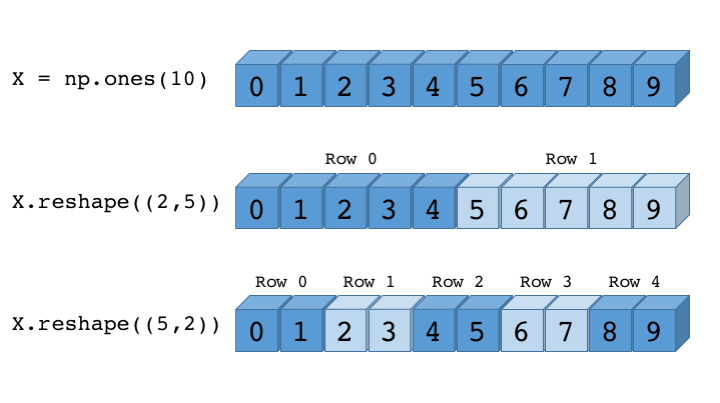
\includegraphics[width=4.5in]{{../Figures/array_slicing/Slide7}.png}
\end{frame}

\begin{frame}[t,fragile]{Shape Manipulation}
	% reshape, resize, ravel, flat, T, -1 for auto reshaping
	Python allows you to specify a \textbf{single} unknown dimension using $-1$.
	\pause
	\begin{lstlisting}
		>>> A = np.arange(6)
		>>> A.
		>>> A.reshape((2,-1))
		array([[0, 1, 2],
		       [3, 4, 5]])
		>>> A.reshape((-1,2))
		array([[0, 1],
		       [2, 3],
		       [4, 5]])
	\end{lstlisting}
\end{frame}

% \begin{frame}[t,fragile]{Shape Manipulation}
% 	% reshape, resize, ravel, flat, T, -1 for auto reshaping
% 	Python allows you to specify a \textbf{single} unknown dimension using $-1$.
% 	\pause
% 	\begin{lstlisting}
% 		>>> A = np.arange(6)
% 		>>> A.reshape((2,-1))
% 		array([[0, 1, 2],
% 		       [3, 4, 5]])
% 		>>> A.reshape((-1,2))
% 		array([[0, 1],
% 		       [2, 3],
% 		       [4, 5]])
% 	\end{lstlisting}
% \end{frame}

% \begin{frame}[t]{Shape Manipulation}
% 	% resize
% \end{frame}

\begin{frame}[t,fragile]{Shape Manipulation}
	% reshape, resize, ravel, flat, T, -1 for auto reshaping
	Other useful functions return specific shapes:
	\pause
	\begin{lstlisting}
		>>> A.ravel()
		array([0, 1, 2, 3, 4, 5])

		>>> A.transpose() # Also use a.T
		array([[0, 3],
		       [1, 4],
		       [2, 5]])
	\end{lstlisting}
\end{frame}

\begin{frame}[t,fragile]{Fancy Indexing}
	% Indexing with arrays of bools
  	NumPy arrays can be indexed with arrays of booleans. This is sometimes called \emph{masking}.
	
	\pause
	\begin{lstlisting}
		>>> A = np.arange(10)
		>>> B = (A%2) == 0
		>>> A[B] # Select all even numbers
		array([0, 2, 4, 6, 8])
		
		>>> A = np.array([[0,-1],[2,3],[-3,2]])
		>>> A
		array([[ 0, -1],
		       [ 2,  3],
		       [-3,  2]])
		>>> B = A.sum(1) < 0
		>>> A[B,:] # Select all rows whose sum is < 0
		array([[ 0, -1],
		       [-3,  2]])
	\end{lstlisting}
\end{frame}

\begin{frame}[t,fragile]{Fancy Indexing}
	% Indexing with arrays of ints
	% Q: what happens to element assignment when index list contains duplicates?
  	Arrays can also be indexed using other \textbf{integer} arrays.
	
	\pause
	\begin{lstlisting}
		>>> A = 2*np.arange(10)
		>>> B = np.array([1,4,5,7])
		>>> A[B]
		array([ 2,  8, 10, 14])
		
		>>> A = np.arange(6).reshape((2,3))
		>>> A
		array([[0, 1, 2],
		       [3, 4, 5]])
		>>> B = np.array([0,0,1])
		>>> C = np.array([1,2,2])
		>>> A[B,C] # One array for each dimension
		array([1, 2, 5])
	\end{lstlisting}
\end{frame}

% \begin{frame}[t]{Interactive Demo}
% \end{frame}

\begin{frame}[t,fragile]{Broadcasting}
	In most cases, when the shapes of two arrays do not match, NumPy will not let you perform elementwise operation between them.
	\pause
	\begin{lstlisting}
		>>> A = np.arange(6).reshape((2,3))
		>>> A
		array([[0, 1, 2],
		       [3, 4, 5]])
		>>> B = np.arange(5)
		>>> A * B
		Traceback (most recent call last):
		  File "<stdin>", line 1, in <module>
		ValueError: operands could not be broadcast together with shapes (2,3) (5,)
	\end{lstlisting}
\end{frame}

\begin{frame}[t,fragile]{Broadcasting}
	In some special cases, NumPy will replicate one or more of the inputs so that it can perform the desired operation. This is called \textbf{broadcasting}.
	\pause
	\begin{lstlisting}
		>>> A = np.arange(6).reshape((2,3))
		>>> A
		array([[0, 1, 2],
		       [3, 4, 5]])
		>>> B = np.arange(3)
		>>> A * B # B is copied for each row of A
		array([[ 0,  1,  4],
		       [ 0,  4, 10]])
	\end{lstlisting}
\end{frame}

\begin{frame}[t]{Broadcasting}
	% Broadcasting 2d
	\centering
	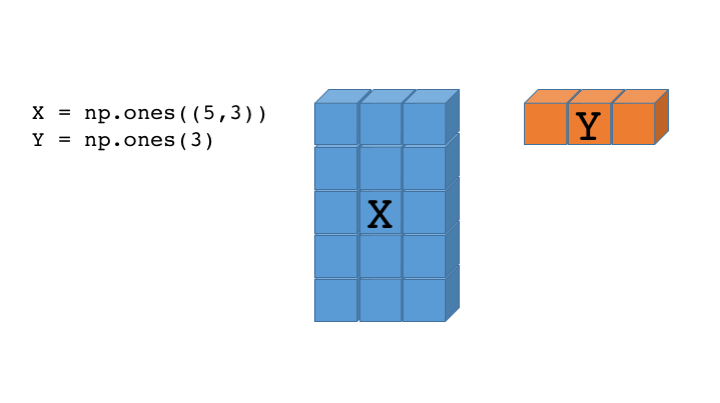
\includegraphics[width=4.5in]{{../Figures/array_slicing/Slide08}.png}
\end{frame}

\begin{frame}[t]{Broadcasting}
	% Broadcasting 2d
	\centering
	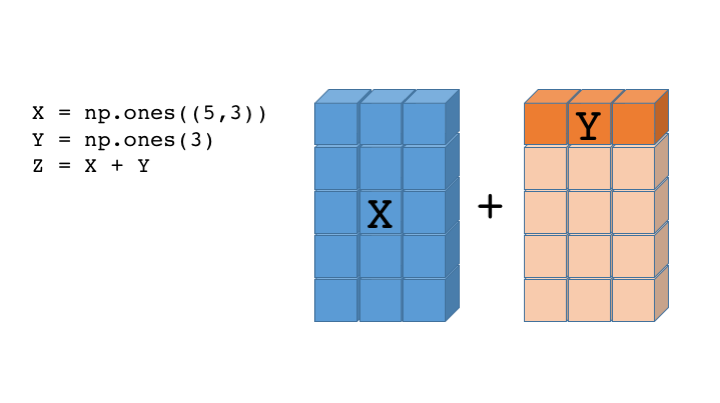
\includegraphics[width=4.5in]{{../Figures/array_slicing/Slide09}.png}
\end{frame}

\begin{frame}[t]{Broadcasting}
	% Broadcasting 2d
	\centering
	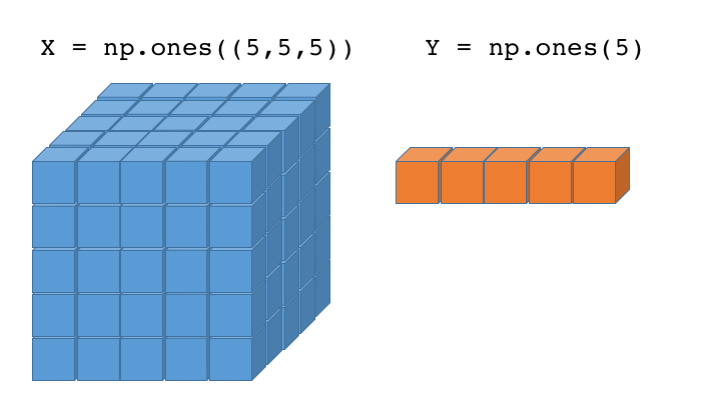
\includegraphics[width=4.5in]{{../Figures/array_slicing/Slide10}.png}
\end{frame}

\begin{frame}[t]{Broadcasting}
	% Broadcasting 2d
	\centering
	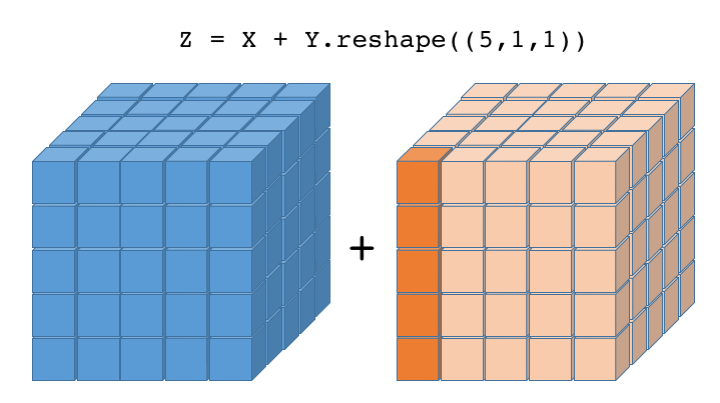
\includegraphics[width=4.5in]{{../Figures/array_slicing/Slide11}.png}
\end{frame}

\begin{frame}[t]{Broadcasting}
	% Broadcasting 2d
	\centering
	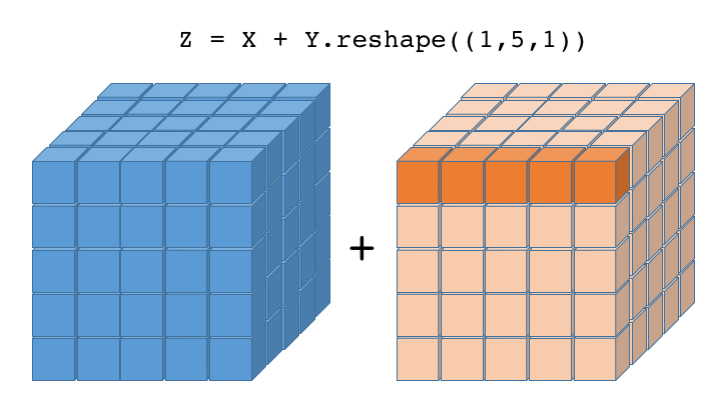
\includegraphics[width=4.5in]{{../Figures/array_slicing/Slide12}.png}
\end{frame}

\begin{frame}[t]{Broadcasting}
	% Broadcasting 2d
	\centering
	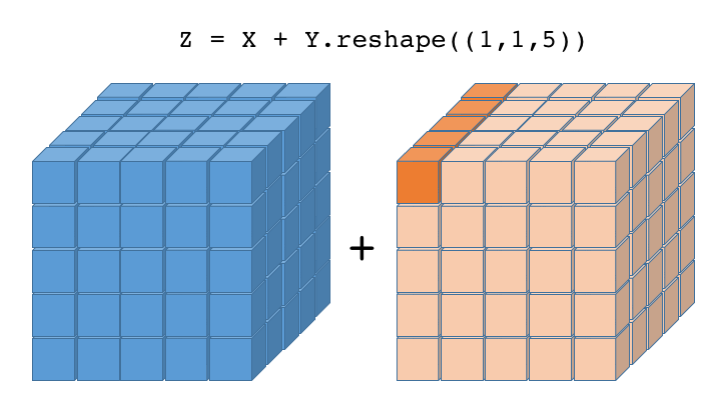
\includegraphics[width=4.5in]{{../Figures/array_slicing/Slide13}.png}
\end{frame}

\begin{frame}[t,fragile]{Interactive Demo}
	\centering
	\Huge{Interactive Demo}
	\normalsize
	\begin{enumerate}
		\item How do you set all of the negative elements in an array to zero?
		\item Recall that you can set an entire slice of an array by using indexed assignment. What happens when assign to a slice indexed by an array and there are duplicates in the \textbf{index} array?
		\begin{itemize}
			\item For example: \verb|a[np.array([1,1,2])] = np.array([1,2,3])|
		\end{itemize}
		\item Use broadcasting to calculate the outer product of two one dimensional arrays (i.e. $A\otimes B = AB^T$).
	\end{enumerate}
\end{frame}

% \begin{frame}[t,fragile]{Interactive Demo}
% 	\centering
% 	\Huge{Interactive Demo}
% 	\normalsize
% 	\begin{enumerate}[<+->]
% 		\item How do you set all of the negative elements in an array to zero?
% 		\begin{itemize}[<+->]
% 			\item \verb|A[A < 0] = 0|
% 		\end{itemize}
% 		\item Recall that you can set an entire slice of an array by using indexed assignment. What happens when assign to a slice indexed by an array and there are duplicates in the \textbf{index} array?
% 		\begin{itemize}
% 			\item It will use that last index
% 		\end{itemize}
% 		\item Use broadcasting to calculate the outer product of two one dimensional arrays (i.e. $A\otimes B = AB^T$).
% 	\end{enumerate}
% \end{frame}
	

% \begin{frame}[t]{Broadcasting}
% 	Example: Broadcasting to calculate an outer product, $\mathbf{a}\mathbf{b}^T$.
% 	\pause
% 	\begin{lstlisting}
% 		>>> a = np.array([1,2,3])
% 		>>> b = np.array([4,5,6])
% 		>>> a.reshape((3,1)) * b.reshape((1,3))
% 		array([[ 4,  5,  6],
% 		       [ 8, 10, 12],
% 		       [12, 15, 18]])
% 	\end{lstlisting}
% \end{frame}


\section{Miscellaneous NumPy}
\subsection{Foo}

\begin{frame}[t,fragile]{Reductions}
	% sum, cumprod, cumsum
	Reductions compute aggregate statistics on the array. For example:
	
	\pause
	\begin{lstlisting}
		>>> A = np.arange(6).reshape((3,2))
		>>> A.sum()
		15
	\end{lstlisting}
\end{frame}

\begin{frame}[t,fragile]{Reductions}
	% sum, cumprod, cumsum
	Most reductions take an argument \verb|axis| which allow you to specify the dimension along which the aggregation takes place.
	
	\pause
	% picture
	\centering
	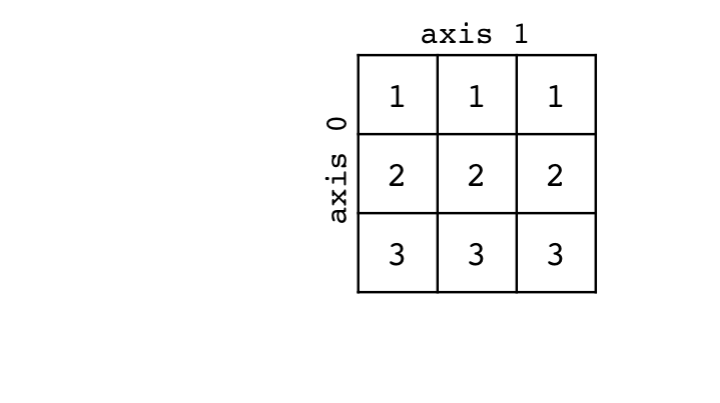
\includegraphics[width=4.5in]{{../Figures/array_slicing/Slide14}.png}
\end{frame}

\begin{frame}[t,fragile]{Reductions}
	% sum, cumprod, cumsum
	Most reductions take an argument \verb|axis| which allow you to specify the dimension along which the aggregation takes place.
	
	% picture
	\centering
	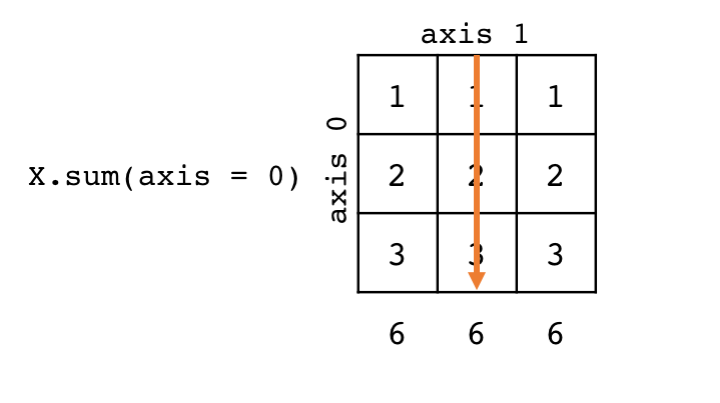
\includegraphics[width=4.5in]{{../Figures/array_slicing/Slide15}.png}
\end{frame}

\begin{frame}[t,fragile]{Reductions}
	% sum, cumprod, cumsum
	Most reductions take an argument \verb|axis| which allow you to specify the dimension along which the aggregation takes place.
	
	% picture
	\centering
	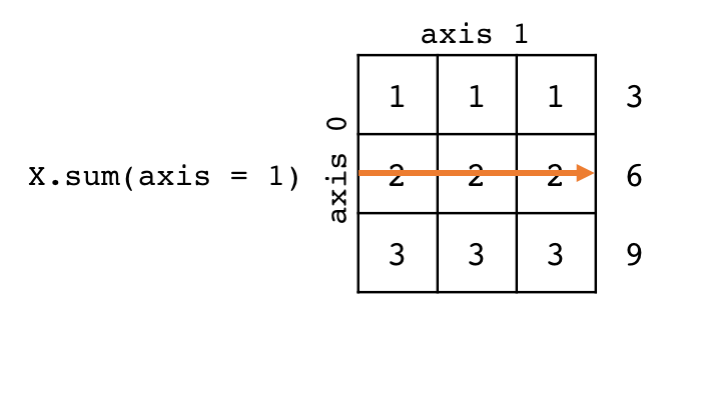
\includegraphics[width=4.5in]{{../Figures/array_slicing/Slide16}.png}
\end{frame}

\begin{frame}[t,fragile]{Reductions}
	% sum, cumprod, cumsum
	Other common reductions are:
	
	\pause	
	\begin{lstlisting}
		>>> A = np.arange(6).reshape((3,2))
		>>> A.prod(axis=0)
		array([ 0,  6, 20])
		>>> A.max(axis=1) # Also min
		array([1, 3, 5])
		>>> A.argmax(axis=1) # Also argmin
		array([1, 1, 1])
		>>> A.mean(axis=1)
		array([ 0.5,  2.5,  4.5])
		>>> A.std(axis=-1) # -1 corresponds to the last dimension
		array([ 0.5,  0.5,  0.5])
		>>> np.median(A,axis=1) # Not a member function
		array([ 0.5,  2.5,  4.5])
	\end{lstlisting}
	% picture
\end{frame}

\begin{frame}[t,fragile]{Stacking}
	% hstack, vstack, column_stack, concatenate
	NumPy provides a number of functions for combining arrays.
	
	\pause
	\begin{lstlisting}
		>>> A = np.ones((3,4))
		>>> B = np.ones((3,4))
		>>> np.vstack((A,B)).shape # first dimension
		(6, 4)
		>>> np.hstack((A,B)).shape # second dimension
		(3, 8)
		>>> np.stack((A,B)).shape # new dimension
		(2, 3, 4)
		>>> np.concatenate((A,B),axis=0).shape # any dimension
		(6, 4)
		>>> np.concatenate((A,B),axis=1).shape # any dimension
		(3, 8)
	\end{lstlisting}
	\pause
	Analogues to each of these functions exist for splitting arrays.
\end{frame}

\begin{frame}[t,fragile]{Copy}
	Because the contents of an array are mutable, we often need to copy the contents of an array to avoid overwriting the original.
	
	\pause
	\begin{lstlisting}
		>>> A = np.ones((3,4))
		>>> B = A
		>>> B is A
		True
		>>> B = A.copy() # Create a new copy of 'A' in memory
		>>> B is A
		False
	\end{lstlisting}
\end{frame}

\begin{frame}[t,fragile]{Basic Linear Algebra}
	% cross, dot, outer, svd, vdot, inv, trace
	NumPy implements many of the standard linear algebra functions:
	
	\begin{itemize}[<+->]
		\item \verb|np.dot(A,B)|: $A^T B$
		\item \verb|np.outer(A,B)|: $A B^T$
		\item \verb|np.trace(A)|: $tr(A)$
		\item \verb|np.inv(A)|: $A^{-1}$
		\item \verb|np.svd(A)|: Singular value decomposition.
		\item And many more...
	\end{itemize}
		
\end{frame}

\begin{frame}[t,fragile]{File I/O}
	NumPy has two main sets of File I/O functions. \verb|load| and \verb|save| read and write .npy files.
	
	\pause
	\begin{lstlisting}
		>>> np.save("my_array.npy",my_array)
		>>> my_array = np.load("my_array.npy")
	\end{lstlisting}
	
	\pause
	\verb|loadtxt| and \verb|savetxt| read and write text files. The \verb|delimiter| argument specifies what character will be used to separate entries and defaults to tab.
	
	\pause
	\begin{lstlisting}
		>>> np.savetxt("my_array.csv",my_array,delimiter=',')
		>>> my_array = np.loadtxt("my_array.npy",delimiter=',')
	\end{lstlisting}
\end{frame}

\begin{frame}[t,fragile]{'Object' Arrays}
	In general arrays store only a single type, however, you can create mixed type arrays by setting the data type to \verb|object|. In python, everything an \verb|object| so these arrays can store anything.
	
	\pause
	\begin{lstlisting}
		>>> A = np.array([1,2.0,"string"],dtype=object)
		>>> A + A
		array([2, 4.0, 'stringstring'], dtype=object)
		>>> A / 3
		Traceback (most recent call last):
		  File "<stdin>", line 1, in <module>
		TypeError: unsupported operand type(s) for /: 'str' and 'int'
	\end{lstlisting}
\end{frame}

\begin{frame}[t,fragile]{Interactive Demo}
	\centering
	\Huge{Interactive Demo}
	\normalsize
	\begin{enumerate}
		\item What is the difference between the reductions \verb|sum| and \verb|cumsum|?
		\item \verb|view()| can be used in a similar way as copy, but has a slightly different effect. Try to figure out what view does.
	\end{enumerate}
\end{frame}
%
%
% \section{Pandas}
% \subsection{Foo}

\end{document}
